\documentclass[a4paper, 12pt]{article}

\usepackage[portuges]{babel}
\usepackage[utf8]{inputenc}
\usepackage[sorting=none]{biblatex}
\addtolength{\textwidth}{1in}
\addtolength{\textheight}{1in}
\addtolength{\evensidemargin}{0.5in}
\addtolength{\oddsidemargin}{-0.5in}
\addtolength{\topmargin}{-0.5in}
\addbibresource{ref.bib}
\usepackage{amsmath}
\usepackage{indentfirst}
\usepackage{graphicx}
\usepackage{multicol,lipsum}

\begin{document}
%\maketitle

\begin{titlepage}
	\begin{center}
	
	%\begin{figure}[!ht]
	%\centering
	%\includegraphics[width=2cm]{c:/ufba.jpg}
	%\end{figure}

		\LARGE{Universidade Federal de Campina Grande}\\
		\large{Departamento de Engenharia Elétrica}\\ 
		\large{Programa de Pós-Graduação em Engenharia Elétrica}\\ 
		\vspace{15pt}
        \vspace{95pt}
        \textbf{\LARGE{Conversores Analógico-para-Informação}}\\
		%\title{{\large{Título}}}
		\vspace{3,5cm}
	\end{center}
	
	\begin{flushleft}
		\begin{tabbing}
			Aluna: Viviane S. G. M. Tenório\\
			Professor: Dr. Raimundo Freire\\
			Disciplina: Instrumentação Eletrônica - 2019.2\\
	\end{tabbing}
 \end{flushleft}
	\vspace{1cm}
	
	\begin{center}
		\vspace{\fill}
			 Novembro\\
		 2019
			\end{center}
\end{titlepage}
%%%%%%%%%%%%%%%%%%%%%%%%%%%%%%%%%%%%%%%%%%%%%%%%%%%%%%%%%%%

% % % % % % % % %FOLHA DE ROSTO % % % % % % % % % %


\newpage
\tableofcontents
\thispagestyle{empty}

\newpage
\pagenumbering{arabic}

\section{Introdução}

A abordagem convencional para amostragem de sinais ou imagens segue o teorema de amostragem de Shannon: a taxa de amostragem deve ser pelo menos duas vezes a frequência máxima presente no sinal (a chamada taxa de Nyquist) \cite{shannon}. De fato, esse princípio está subjacente a quase todos os protocolos de aquisição de sinal usados em eletrônicos visuais e de áudio do consumidor, dispositivos de imagem médica, receptores de rádio e assim por diante. No campo da conversão de dados, por exemplo, a tecnologia padrão de conversor analógico-digital (ADC) implementa a representação quantificada usual de Shannon: o sinal é amostrado uniformemente na taxa de Nyquist ou acima dela.

Com a crescente tendência em direção a sistemas de monitoramento de saúde vestíveis, uma grande quantidade de dados é continuamente coletada, armazenada, transmitida e processada para extrair informações essenciais de diferentes sinais fisiológicos. Esses requisitos provam ser uma grande restrição para aplicações móveis ou ambulatoriais, onde o baixo consumo de energia é um pré-requisito.
Sistemas que podem compactar o número de amostras de dados coletadas diretamente na fonte enquanto capturam simultaneamente os principais recursos do sinal reduzirão significativamente a carga de energia e os requisitos de armazenamento. Maior compactação e extração direta de recursos são os principais objetivos de design para esses aplicativos.
A compressão Wavelet foi sugerida para reduzir a quantidade de dados necessários para representar os sinais fisiológicos. No entanto, ainda é necessário adquirir uma grande quantidade de dados na taxa de Nyquist que é compactada posteriormente.

Isso coloca uma carga a mais nos requisitos de armazenamento em tempo real. Os recentes desenvolvimentos em uma abordagem de sensoriamento comprimido foram comprovados serem muito eficazes para a compactação de dados. O \textit{framework} do \textit{compressed sensing} permite amostragem e digitalização em taxas muito inferiores à taxa de Nyquist e permite reconstrução do sinal. 

Ele basicamente reconhece que a maioria dos sinais de entrada é escassa em algum conjunto de bases. Um desses exemplos de interesse é a amostragem do sinal de entrada em um conjunto de bases diferente do próprio da entrada (por exemplo, amostragem aleatória), seguida pelo pós-processamento digital para reconstruir o sinal usando uma restrição métrica, como a norma. 

O \textit{compressed sensing} também foi usado para aplicações, como imagens de pixel único e imagens médicas de Ressonância Magnética. No entanto, as complexas tarefas de pós-processamento digital para a reconstrução de sinais tornam todos esses sistemas inviáveis para aplicações de detecção biomédica e implantável.

Uma abordagem alternativa para a compactação de fonte é o esquema de amostragem assíncrona determinística, que digitaliza o sinal de entrada com base em seu nível de atividade. Tsividis \cite{tsividis1986continuous} demonstrou ainda mais sua utilidade no contexto de processadores de sinais digitais de tempo contínuo. 

Para alcançar níveis ainda mais altos de compactação de dados e economia de energia, um esquema de amostragem assíncrona adaptativo, que utiliza as informações sobre a inclinação do sinal de entrada para ajustar a resolução do quantizador embutido.

A abordagem assíncrona adaptativa fornece compressão significativa para muitos sinais fisiológicos que são relativamente escassos e demonstram comportamento semelhante a uma explosão, como eletrocardiogramas (ECG), sinais eletroencefalográficos (EEG) e potenciais de ação dos neurônios

\section{Fundamentação Teórica}

A prevalência do processamento de sinal digital em aplicativos de comunicação popularizou o uso dos conversores analógico-digital (ADC). Esses ADCs empregam o teorema de amostragem Nyquist, que garante a reconstrução de um sinal de banda limitada quando ele é amostrado uniformemente com uma taxa de pelo menos duas vezes sua largura de banda.

Consequentemente, é necessário um número excessivamente grande de amostras para representar sinais de banda larga, exigindo grandes quantidades de recursos para armazenar e transmitir esses dados. Aplicativos emergentes, como detecção de radar e comunicação de banda ultra-larga, estão levando o desempenho dos ADCs para seus limites físicos.

Em muitos casos de interesse, os sinais têm estrutura adicional, além da limitação de banda. Nos últimos anos, surgiu uma teoria baseada na amostragem compressiva -- o \textit{Compressed Sensing} (CS) -- que explora esse conhecimento para obter reconstrução de sinal usando menos medições que o número prescrito pelo teorema de Nyquist para certas classes de sinais. 

Em particular, o CS permite a reconstrução de sinais que são compressíveis por alguma transformação, o que significa que a representação da transformação tem alguns coeficientes grandes e muitos coeficientes pequenos.

\subsection{Amostragem Compressiva}

A teoria da amostragem compressiva afirma que é possível recuperar certos sinais e imagens a partir de muito menos amostras ou medições do que os métodos tradicionais usam. Para tornar isso possível, a amostragem compressiva se baseia em dois princípios: a esparsidade, que pertence aos sinais de interesse, e a incoerência, que pertence à modalidade de detecção.

\begin{itemize}
    \item A \textbf{esparsidade} expressa a ideia de que a ``taxa de informação'' de um sinal de tempo contínuo pode ser muito menor do que o sugerido por sua largura de banda, ou que um sinal de tempo discreto depende de vários graus de liberdade que são comparativamente muito menores que seu (finito) comprimento. Mais precisamente, a amostragem compressiva explora o fato de que muitos sinais naturais são escassos ou compressíveis no sentido de que eles têm representações concisas quando expressos na base adequada $\Psi$.
    \item A \textbf{incoerência} estende a dualidade entre tempo e frequência e expressa a ideia de que objetos com uma representação esparsa em be devem ser espalhados no domínio em que são adquiridos, assim como um Dirac ou um pico no domínio do tempo é espalhado na frequência domínio. Em outras palavras, a incoerência diz que, diferentemente do sinal de interesse, as formas de onda de amostragem / detecção têm uma representação extremamente densa em $\Psi$.
\end{itemize}{}

É importante destacar que é possível projetar protocolos de detecção ou amostragem eficientes que capturam o conteúdo de informação útil incorporado em um sinal esparso e o condensam em uma pequena quantidade de dados.

Esses protocolos não são adaptativos e apenas demandam a correlação do sinal com um pequeno número de formas de onda fixas que são incoerentes com a base, oferecendo uma descrição concisa do sinal. (Caso contrário, não há dependência do processo de medição no próprio sinal.) 

Em outras palavras, o \textit{Compressed Sensing} é um protocolo de aquisição de sinal muito simples e eficiente, que coleta amostras - de maneira independente de sinal - a uma taxa baixa e, posteriormente, utiliza energia computacional para reconstrução do que parece ser um conjunto incompleto de medições.

\subsection{Estado da Arte}

A amostragem compressiva surgiu nos últimos 10 anos em decorrência do grande volume de dados obtidos por meio do sensoriamento. Com o amplo uso de sensores mais baratos, sistemas embarcados e -- mais recentemente -- dispositivos \textit{IoT} (Internet das Coisas), percebeu-se que o volume de dados era inconsistentes com a quantidade de informação disponível nos mesmos. Ou seja, muito processamento estava sendo utilizado para pouca informação. Os trabalhos a seguir apresentam soluções, discutem aspectos práticos e teóricos, bem como propõe novos paradigmas para a implementação física do \textit{Compressed Sensing}: os conversores analógico para informação.

O artigo \cite{wadhwa2016slicer} possui um estudo interessante sobre o ADC espaçado por símbolos padrão com severas restrições de quantização, em que se estime o número mínimo de \textit{slicers} necessários para evitar erros. Observa-se que \textbf{o desempenho é sensível à fase de realização e amostragem de canais}, o que motiva uma arquitetura espaço-temporal mais flexível. As arquiteturas propostas (baseadas em CS) não têm limitações fundamentais na teoria: dispersar aleatoriamente \textit{slicers} suficientes de um bit no espaço e no tempo fornece informações suficientes para uma equalização confiável. Projetos práticos para amostragem com espaçamento de símbolos foram apresentados, além de propor um algoritmo para otimizar os limiares de \textit{slicer}, o que melhora significativamente o desempenho em relação a um \textit{design} padrão.

Em \cite{shen2017design}, é proposta uma solução de hardware para aquisição e processamento de sinal em nós finais de Redes de Sensores Sem Fio. Propõem o paradigma de um conversor de analógico para informação (AIC) baseado na teoria de \textit{Compressed Sensing} (CS). O modelo do sistema consiste em um módulo de modulação, módulo de filtragem e módulo de amostragem. Além disso, é apresentado o design do hardware e a implementação de um sistema AIC digital aprimorado. Também foi estudado o desempenho de três algoritmos de recuperação de dados gananciosos diferentes e analisados quanto ao consumo de energia do sistema. Os resultados experimentais mostram que, para sinais ambientais normais, o novo sistema supera o limite de Nyquist e exibe bom desempenho de recuperação com baixa frequência de amostragem, o que é adequado para o monitoramento ambiental baseado em Redes de Sensores sem Fio.

O trabalho de \cite{pelissier2017non} propõe uma nova arquitetura AIC baseada em CS chamada \textbf{amostragem não-uniforme de \textit{wavelets} (NUWS)}. A solução extrai um subconjunto cuidadosamente selecionado de coeficientes de \textit{wavelet} diretamente no domínio RF, o que mitiga os principais problemas das arquiteturas de conversor AIC existentes. Para sinais de RF de banda múltipla, propõe-se uma variante especializada chamada de \textbf{amostragem não uniforme em banda-base de \textit{wavelet} (NUWBS)}, que melhora ainda mais a sensibilidade e reduz a complexidade do hardware, alavancando a estrutura do sinal de banda múltipla. Simulações demonstram que o NUWBS se aproxima dos limites teóricos de desempenho da recuperação de sinais esparsos baseados em norma 1. Aspectos de design de hardware foram investigados e foram apresentados resultados de medição de um \textit{Application-specific integrated circuit} (ASIC) para o estágio de geração de \textit{wavelets}, que destacam a eficácia do NUWBS para uma ampla gama de tarefas de extração de recursos de RF em aplicações com custo e energia limitados.

Em seu trabalho mais recente, \cite{pelissierexperimental}, os autores apresentaram resultados experimentais da solução \textbf{NUWS} para aplicações de rádio cognitivo. O ASIC explorado realiza aquisição compressiva com consumo de energia tão baixo quanto $225$ $pJ/medida$ para um sinal de RF na faixa de GHz. Um gráfico experimental de transição de fase é relatado com uma comparação com sua contraparte teórica.

No artigo \cite{silva2018testing}, um método de teste é adaptado e aplicado para avaliar uma implementação física de uma arquitetura configurável AIC baseada no RMPI \textit{(Random Modulation Pre-Integrator}). Por meio desse método de teste, é possível obter a relação sinal-ruído e distorção (SINAD) diretamente da saída AIC sem o uso do algoritmo de reconstrução de sinal. Este método de teste foi validado para esta arquitetura por simulações e por experimentação em hardware. Os resultados mostram que alguns recursos podem ser extraídos por meio do SINAD, como a melhor faixa de amplitude do sinal de entrada a ser usada e quais parâmetros configuráveis melhor se ajustam ao conversor.

O hardware do AIC sofre de não idealidades de componentes e subsistemas, o que reduz a qualidade da reconstrução do sinal medido. Tais efeitos podem ser compensados pela calibração que normalmente foi implementada nos métodos de recuperação de sinal. No artigo \cite{ws2018gain}, é analisado um método de calibração para o AIC que leva em consideração apenas as medidas produzidas pelo AIC. Os resultados mostram que a calibração do hardware melhora a reconstrução do sinal em relação à relação sinal-ruído e distorção (SINAD), independentemente do algoritmo de reconstrução.


O artigo em \cite{zeng2019interception} descreve um tipo de esquema de informação analógica que consiste em desmodulação, filtragem e amostragem uniforme. Com base no esquema, os sinais de modulação de frequência senoidal e linear (LFM) podem ser reconstruídos e os resultados mostram que o esquema AIC aliviaria o problema da alta taxa de amostragem. O sinal pode ser reconstruído com precisão quando é amostrado com um fator de subamostragem 0,2.

O trabalho em \cite{lopez2019analog} apresenta o \textit{design} e a implementação de um conversor de analógico para informação (AIC) de 100 MHz, baseado no demodulador aleatório. Para tal, foram utilizados componentes \textit{``de prateleira''} para implementar o \textit{front-end} analógico, e um chip SoC-FPGA para implementar o subsistema de hardware / software digital. 
O front-end analógico é composto por um misturador e um filtro passa-baixas, que foram implementados usando uma Célula de Gilbert e um circuito RC passivo, respectivamente. O subsistema de hardware / software foi com um chip SoC-FPGA, onde o lado FPGA foi usado para implementar o hardware que gerencia o lado RD e HPS foi usado para implementar algoritmos de recuperação de espectro. Finalmente, os resultados da verificação mostraram que o AIC projetado pode recuperar sinais esparsos de largura de banda de 100 MHz, onde uma taxa sub-Nyquist de 4 MHz é usada junto com dois algoritmos de recuperação de Sensoriamento Compressivo (CS).

No trabalho \cite{silva2019novel}, dois novos métodos de teste AIC são introduzidos, nos quais apenas as saídas AIC, ou seja, apenas as saídas compactadas $y$, são levadas em consideração. No primeiro, podem ser aplicados sinais multi-seno e, no segundo, métodos de ajuste de onda senoidal de quatro parâmetros, conforme recomendado pela Norma 1241 da IEEE. Resultados experimentais foram obtidos para duas implementações diferentes da AIC (a saber, desmodulador aleatório e pré-integrador de modulação aleatória) e a relação sinal-ruído e distorção (SINAD) de ambas foi medida diretamente a partir da saída da AIC, provando que os métodos de teste da AIC propostos são eficazes.



\section{Conversores AI}

Entende-se por conversor analógico para informação (AIC) é o responsável pelo processo de aquisição, a partir da Amostragem Compressiva, do sinal analógico. O objetivo de um AIC é efetuar a digitalização de sinais de maneira eficiente, visando a economia em taxa de amostragem e em capacidade de armazenamento, bem como superar o desempenho e as limitações de eficiência energética dos conversores analógicos-digital \cite{Bruno2019}. 

A denominação AIC vem da sua capacidade de adquirir não o sinal, mas
a informação contida nele \cite{daponte2017analog}. O sistema pode ser visto como um instrumento de medição constituído por duas partes: 
\begin{itemize}
    \item um front-end analógico, formado por um conversor analógico para informação (AIC);
    \item um back-end digital (ou seja, hardware de processamento de sinal digital), onde um algoritmo de reconstrução de sinal é utilizado.
\end{itemize}

Partindo da teoria da amostragem compressiva, dado um sinal $x \in I\!R^n$ com $m$ medições lineares, pode ser representado matematicamente por:

\begin{equation}
    y = Ax
\end{equation}{}

onde A é uma matrix $m \times n$ e $y \in I\!R^m$. A matriz A representa a redução de dimensionalidade  -- ou seja, mapeia $I\!R^n$ ($n$ geralmente é grande) em $I\!R^m$, em que $m$ é tipicamente bem menor que $n$.

Na prática, essa operação é realizada em um intervalo finito $t \in [0,T]$, pois o sinal a ser adquirido está no tempo contínuo, conforme a expressão a seguir.

\begin{equation}
    y_m = \int_0^T x(t) A_m(t) \mathrm{d}x
\end{equation}{}

em que $x(t)$ é o sinal de entrada e $A_m(t)$ são funções para as realizações das medições. Pela expressão acima, observa-se que para um AIC adquirir um sinal $x(t)$ são necessários elementos multiplicativos e integrativos. Além disso, para uma implementação prática, serão necessários: um dispositivo que gere sequências pseudo-aleatórias e um dispositivo para digitalizar as medidas do vetor $y$, \cite{Bruno2019}.

Logo, as arquiteturas propostas atualmente que serão apresentadas a seguir, são diferenciadas pelo modo de operação e o tipo de cada um desses dispositivos.

\subsection{Demodulador Aleatório}

O demodulador aleatório (do inglês, \textit{Random Demodulator}) baseia-se na correlação do sinal de entrada $x(t)$ com uma sequência binária pseudo-aleatória com amplitudes de valores $\pm1$, resultando em um espalhamento espectral.
Em seguida, o sinal é aplicado num filtro passa-baixas e capturado por um conversor analógico-digital (ADC) com uma taxa de amostragem menor do que a de Nyquist.
A Figura \ref{fig:fig1} apresenta o diagrama de blocos para o demodulador aleatório como proposto em \cite{dutta2015analog}.

\begin{figure}[h!]
    \centering
    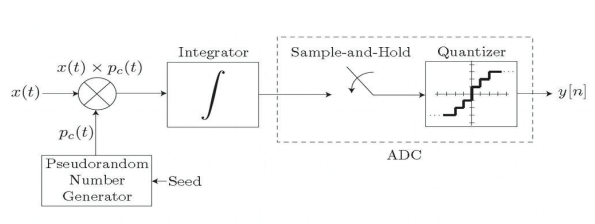
\includegraphics[scale=0.85]{fig1.PNG}
    \caption{Diagrama de blocos para o demodulador aleatório. (Fonte:  \cite{dutta2015analog}.)}
    \label{fig:fig1}
\end{figure}{}

Segundo \cite{tropp2009beyond}, o espalhamento espectral é visto como uma assinatura do sinal, ou seja, para uma mesma sequência $p_c(t)$ cada sinal terá um formato próprio depois da multiplicação\cite{Vanderson2017}. 

Assim, o demodulador aleatório apresenta baixa complexidade de implementação, contudo suporta apenas a reconstrução de sinais multi-tom discreto. 

\subsection{Amostrador Não-uniforme}

O Amostrador Não Uniforme (do inglês, \textit{Non-Uniform Sampler}) consistem em uma maneira de digitalizar a informação de sinais que são esparsos no domínio da frequência. 

O sinal $x(t)$ é digitalizado por um ADC que trabalha na taxa de Nyquist. O sinal já digitalizado vai para um seletor que através de uma sequência
aleatória define se o valor é descartado ou mantido.

Dessa forma, a implementação de um NUS necessita de um conversor A/D, um
gerador de sequências aleatórias e uma chave seletora. Nos trabalhos de \cite{bellasi2013vlsi} e \cite{pelissier2017non} vemos implementações dessa variação de AIC. Na figura \ref{fig:fig2} é possível observar o diagrama de blocos de um amostrador não-uniforme.

\begin{figure}[h!]
    \centering
    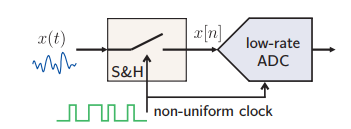
\includegraphics{fig2.PNG}
    \caption{Diagrama de blocos da arquitetura NUS (Fonte: \cite{pelissier2017non}.)}
    \label{fig:my_label}
\end{figure}{}

Se a subamostragem é aleatória, não há efeito de recobrimento coerente e os sinais esparsos na frequência podem ser recuperados por meio de processamento não-linear \cite{daponte2016prbs}.

\subsection{Conversor de Banda Larga Modulada}

O Conversor de Banda Larga Modulada é uma arquitetura paralela, em que cada elemento paralelo é chamando de canal \cite{Vanderson2017}. O sinal de entrada $x(t)$ é do tipo RF multibanda, assim cada canal recebe o mesmo sinal RF de entrada e mistura com uma forma de onda distinta para cada canal. O número de canais depende da taxa de amostragem em cada canal.

A operação de modulação projeta o espectro de $x(t)$, de modo que uma parte da energia de todas as bandas apareça na banda base. Entretanto, a periodicidade das sequências pseudoaleatórias implica que elas podem ser expandidas em uma série de Fourier, o que garante que o recobrimento (\textit{aliasing}) do sinal $x(t)$ aconteça nos pontos de cruzamento entre as bandas resultando em um processo de amostragem tradicional por trem de pulsos na taxa $F_s$ \cite{Bruno2019}.

Esse sinal na banda base passa por um filtro passa-baixas e um ADC de taxa baixa por canal, da mesma forma que as demais arquiteturas. 

\subsection{Pré-Integrador de Modulação Aleatória}

O Pré-Integrador de Modulação Aleatória (RMPI) possui características tanto da arquitetura do Demodulador Aleatório como do Conversor de Banda Larga Modulada. 

O RMPI possui a mesma estrutura paralela do Conversor de Banda Larga Modulada, contudo usa um circuito integrador semelhante ao do Demodulador Aleatório, conforme Figura \ref{fig:fig3}. 

\begin{figure}[h!]
    \centering
    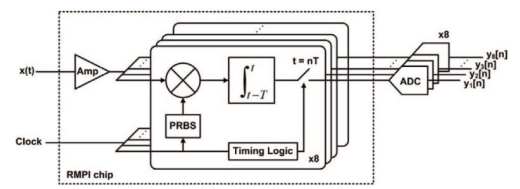
\includegraphics{fig3.PNG}
    \caption{Diagrama em bloco do RPMI. (Fonte: \cite{Vanderson2017}.)}
    \label{fig:fig3}
\end{figure}{}

Cada canal possui um multiplicador que funciona como um
\textit{down-converter} que usa um Sequência Binária Pseudo-Aleatória ao invés de um oscilador. Essas sequências são usadas por serem incoerentes com qualquer base estruturada. Segundo Reis \cite{Vanderson2017}, essa arquitetura é relativamente universal pois funciona com sinais que são esparsos em qualquer domínio fixo. 


\section{Discussões e Conclusões}

Por se tratar de um tema relativamente recente, os conversores AIC estão em constante desenvolvimento. Ao longo da revisão bibliográfica foi possível observar que as principais arquiteturas de AIC são baseadas em um modelo linear e basicamente consistem de multiplicadores, geradores de sequências pseudoaleatórias, filtros passa-baixas e ADC de baixa taxa de amostragem. 

Esses componentes inserem não-linearidades no hardware do AIC e, dependendo da forma como são utilizados, comprometem a reconstrução do sinal. Além disso, os efeitos de \textit{jitter} e abertura, no estágio de mistura dos sistemas AIC limitam sua resolução e desempenho.

A sensibilidade da reconstrução é parcialmente devida ao fato de que esses
comportamentos reduzem a viabilidade do sistema no sentido de CS, mas também porque durante a reconstrução não se pode produzir uma matriz que esteja exatamente sintonizada com as não idealidades -- algumas das quais são de natureza estocástica.

Apesar das atuais limitações, diversas aplicações em imagens médicas (fMRI e a ressonância magnética convencional), radares e até em segurança asseguram não só sua viabilidade física como também sua importância nos dias atuais.

Abordagens recentes trazem como sugestões de trabalhos futuros arquiteturas que minimizem os efeitos da não-linearidade dos componentes, bem como técnicas lineares para sinais ``quase-esparsos'' -- dado que nem sempre os sinais podem ser completamente categorizados como esparsos.

\clearpage
\printbibliography
\end{document}



